%!TEX root = thesis.tex
\chapter{Introduction}
\label{cha:introduction}

Ever since the dawn of time, the humankind have looked at the stars and wondered if we are alone in
this Universe. To answer this question, one must look toward the field of extrasolar planets
(exoplanets). This is a rapidly growing field in astronomy and science in general. Ever since the
first confirmed discovery of an exoplanet around a millisecond pulsar in 1992 by
\citet{Wolszczan1992} and three years later, the more interesting exoplanet 51 Peg b discovered
around a solar-type star by \citet{Mayor1995}, more than 3600 exoplanets have been discovered at the
time of writing, July 2017\footnote{\url{http://exoplanet.eu/}}.

With the discoveries of exoplanets, the main focus is now mainly on finding the twin of Earth, that
is a planet that can harbour life as we know it. However, in order to accurately and precisely
characterise an exoplanet, it is is crucial to characterise its host star. This is commonly known as
``know the star, know the exoplanet''. It is possible to obtain planetary global parameters such as
its radius and mass if the stellar parameters are accurately known. With high precision it is even
possible to distinguish between different planetary bulk compositions such as water-worlds, rocky
planets, gaseous planets, iron planets, or exotic combinations of the above.

In this chapter there will be a general introduction to exoplanets, detection methods, and
characterisation (\sref{sec:exoplanets}). Then a throughout introduction on the exoplanet host
stars (\sref{sec:planet_host_stars}), which is the main focus on this thesis. While learning about
host stars, and stars in general, the results have wide-spread applications, where some will briefly
be discussed in the end of this chapter (\sref{sec:stars_application}) before an introduction on
what this thesis will consists of (\sref{sec:this_thesis}).



\section{Exoplanets}
\label{sec:exoplanets}

The holy grail in the field of exoplanets is to find the first exoplanet with life. This is by no
means an easy task. To give an idea of the difficulty of detecting life on an exoplanet, one must
understand all the difficulties to simply detect and confirm an exoplanet. This will shortly be
described in the sections below where several detection techniques will be introduced.

\subsection{Detecting exoplanets}
\label{sec:detecting_exoplanets}

There are six main techniques of detecting exoplanets, some with advantages over others. A lot of
information about the exoplanets can be extracted when more than one of techniques are used and
combined.

It is important to note, that different things might mimic planetary signals, such as stellar
activity, the light from a lighter stellar companion \citep[see e.g.][]{Oshagh2013,Oshagh2014}.
However they will not be described in this thesis. Two techniques are often combined in order to
confirm the detection of an exoplanet.

The description of the different detection techniques are inspired by \citet{Seager2010}.


\subsubsection{Transit method}
\label{sec:transitMethod}

The most successful method, if based on numbers of exoplanets detected, is the transit method. This
is a well-known method in astronomy, however only used recently for detecting exoplanets. Before
this, it has been used extensively for finding and characterising eclipsing binary stars. The
difference here is, that the exoplanet is extremely small and does not radiate (or at least emit
very little radiation). An example of an exoplanet transiting a star can be seen in
\fref{fig:transitMethod}.

\begin{figure}[htpb!]
    \centering
    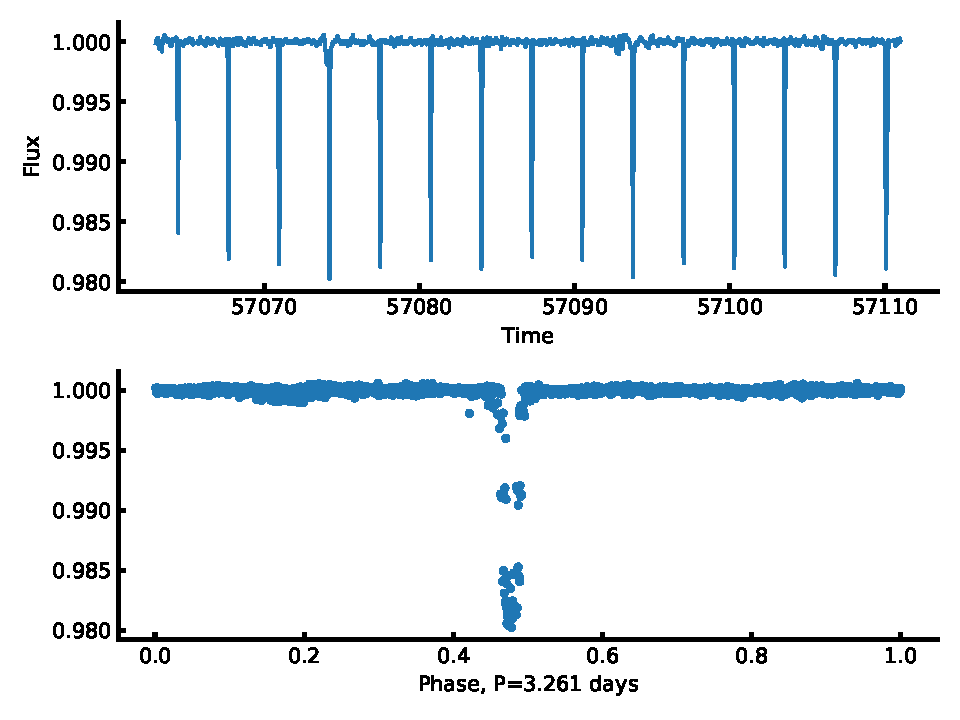
\includegraphics[width=1.0\linewidth]{figures/transitMethod.pdf}
    \caption{\emph{Upper plot}: The lightcurve of a star with an exoplanet transiting.
             \emph{Lower plot}: The phase curve of the above lightcurve.}
    \label{fig:transitMethod}
\end{figure}

As an exoplanet transits its host star, the total brightness from the system will decrease, as the
exoplanet blocks some of the light from the star. This dimming in brightness will be seen
periodically as the exoplanet orbits its host star. The decrease in brightness as the planet transit
the star is directly related to ration between the stellar radius $R_\ast$ and the planetary radius
$R_p$:
\begin{align}
  k = \sqrt{\frac{R_p}{R_\ast}},  \label{eq:transit}
\end{align}
where $k$ is the depth of the transit compared to the total stellar brightness.

It is possible to obtain the radius of an exoplanet with this method. However, detailed analysis of
the phase curve of an exoplanet can additionally reveal the surface temperature of the exoplanet.
The transit described above is also known as the primary transit. If it is possible to detect the
secondary transit, that is when the exoplanet goes behind the star as seen from Earth, the
difference in light (planet + star right before secondary transit compared to just star) gives the
flux of the planet and thus the surface temperature. This is a difficult task as secondary transits
are intrinsic faint.


\subsubsection{Radial velocity method}
\label{sec:rvmethod}

The radial velocity method is the indirect study of the motion of the host star using the Doppler
effect caused by an orbiting exoplanet. This together with the transit method described above are by
far the most successful methods to detect and characterise exoplanets. The periodic signal created
by the exoplanet on the host star depends on the mass ratio between the star $M_\ast$ and the planet
$M_p$:
\begin{align}
  K = \frac{\SI{28.4329}{km/s}}{\sqrt{1-e^2}} \frac{M_p\sin i}{\Mjup} \left( \frac{M_\ast+M_p}{M_\odot} \right)^{-2/3} \left(\frac{P}{\SI{1}{year}}\right)  \label{eq:rv}
\end{align}
where $K$ is the semi-amplitude of the sinusoidal, $e$ is the eccentricity, $i$ is the inclination,
$P$ is the orbital period, and $\Mjup$ is the mass of Jupiter. Since $M_\ast \gg M_p$, the term
$M_\ast+M_p\simeq M_\ast$ in order to simplify the equation. Often a circular orbit is assumed,
$e=0$. The sinusoidal motion of the star can be seen in \fref{fig:rvmethod} where both the time
series and the phase curve is presented for an exoplanet.

\begin{figure}[htpb!]
    \centering
    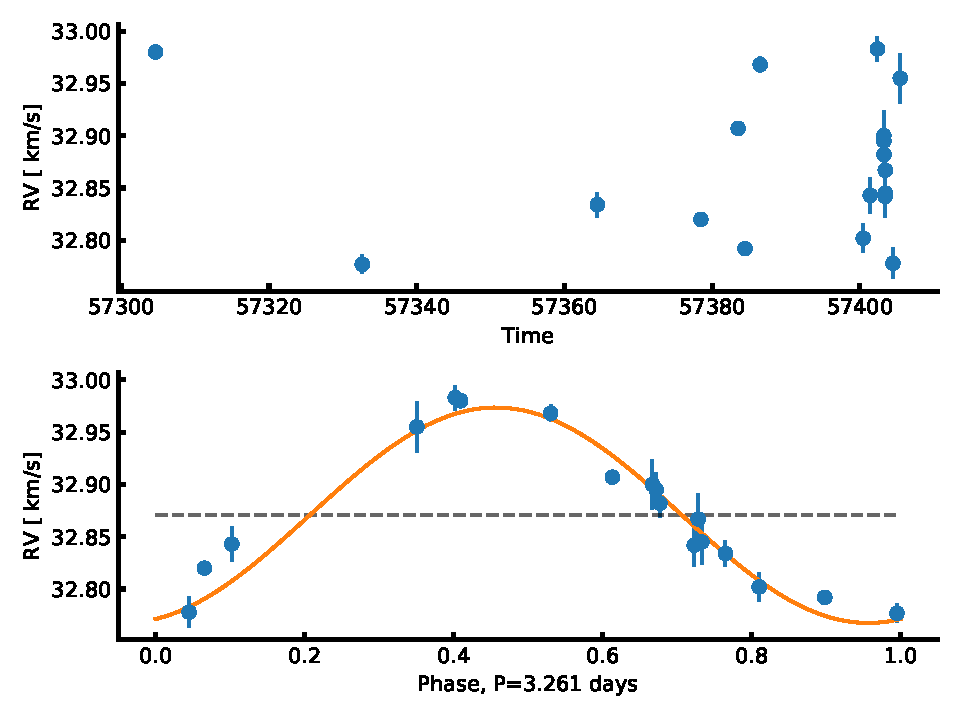
\includegraphics[width=1.0\linewidth]{figures/RVmethod.pdf}
    \caption{\emph{Upper panel}: RV time series of EPIC 9792 from the SOPHIE spectrograph.
             \emph{Lower panel}: Phase curve of the time series above, using the period of
             \SI{3.261}{days}.}
    \label{fig:rvmethod}
\end{figure}

In order to apply the radial velocity method for detecting exoplanets, it is necessary to collect
spectra (high resolution but often not high S/N) in order to cover most part of the phase of the
orbit. These spectra are often combined after the detection of the exoplanet, in order to increase
the S/N. This combined spectrum can then be used for characterising the host star.


\subsubsection{Other techniques}

The following four techniques have all detected exoplanets, however, they are not widely used and
neither has the same level of success as the two methods described above.

\paragraph{Direct imaging}

Direct imaging is probably the easiest method to understand, however it is quite difficult to
actually use this technique. In its core, by carefully blocking the light of a star, it is possible
to directly image the exoplanets around it. However, it is extremely difficult to block the light
of the host star and find the reflected light of the exoplanet(s) in orbit.

This technique is sensitive to exoplanets which reflect a lot of light, i.e. a high albedo, and in
wide orbits as they are less contaminated by the residual starlight.

\paragraph{Astrometry}

Using astrometry to detect exoplanets is very similar to the RV method described above in
\sref{sec:rvmethod}. Here by carefully detecting the minute motion of a star caused by an
exoplanet. Unlike the RV method, this technique (astrometry) actually looks for changes in the
coordinates of the star.

This technique is sensitive to massive exoplanets as they cause a larger motion compared to lighter
companions.


\paragraph{Transit timing variation}

This technique of detecting exoplanets is a highly indirect method of detecting exoplanets. Here an
a transiting exoplanet has to be detected first as explained in \sref{sec:transitMethod}. Then
variations in the occurrence of mid-transit can be detected if a second non-transiting exoplanet
interact with the primary transiting exoplanet (planet-planet interaction). This interaction will
periodically course the mid-transit to happen ahead/behind of the time if only one exoplanet would
be present.

A careful analysis of the transit timing variations (TTV) can give the mass of the secondary
non-transiting exoplanet. However, its radius will be unknown. Most of these exoplanets pairs which
shows TTV are in an orbital resonant. This technique as well, is more sensitive to massive
exoplanets as they will induce a higher signal.


\paragraph{Microlensing}

This technique is very exotic and not widely used, however since a few exoplanets have been
discovered by this technique it deserves a mentioning. The core theory in this technique is the
well-known General Relativity by \citet{Einstein1916}. Here an observer looks at a distant star
(star A) as a star between the observer and the distant star (star B) passes in between the line of
sight. Star B will act as a lens and increase the magnitude of star A. This increase of magnitude
will reach its maximum as the two stars are most aligned as seen from Earth.

To use this for detecting exoplanet, there will have to be an exoplanet orbiting star B. This act as
a microlens, momentarily make a secondary increase in magnitude. The amount of increase in magnitude
is related to the mass of the exoplanet. The higher the mass, the higher the effect.

While this exotic technique is interesting and has proven successful, it is not very useful as it
only occurs once. The stars observed with this technique are often faint, thus making follow-up RV
detection very difficult if not impossible with the current instruments.


\subsection{Towards the Earth twin}

The above mentioned techniques will be used to find the Earth twin. Especially will the two first
techniques (transit and RV method) be the ones finding the smallest exoplanets as a wide range of
instruments are being developed dedicated for this\unfinished{Write about JWST, Espresso, NIRPS,
etc.}. Since the detection of the first exoplanet around a solar-type star by \citet{Mayor1995}, the
community has been able to detect lower mass exoplanets as seen in \fref{fig:exoplanetMass}.

\begin{figure}[htpb!]
    \centering
    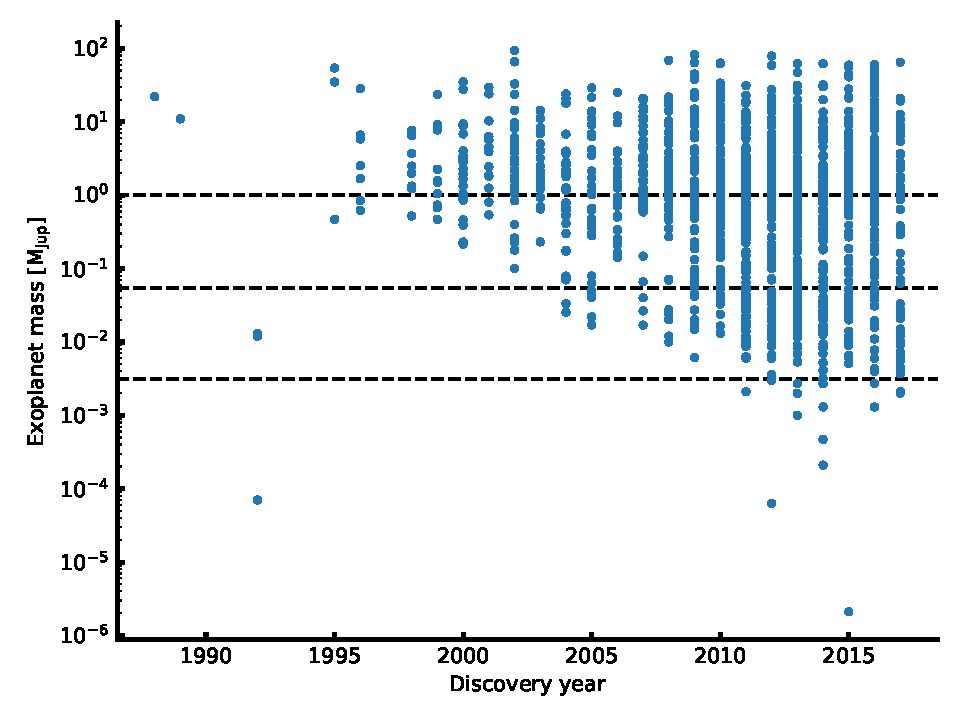
\includegraphics[width=0.8\linewidth]{figures/exoplanetMass.pdf}
    \caption{The mass of exoplanet since the detection of the first exoplanet until now. The
             horizontal lines are the mass of Jupiter (upper), Neptune (middle), and Earth (lower).}
    \label{fig:exoplanetMass}
\end{figure}

While the first many discoveries of exoplanets were the, at the time, exotic and strange hot
Jupiter-like exoplanets in close orbits, the time have come to detect exoplanets with both lower
mass and wider orbits. It is crucial to have high precision instruments and long surveys to detect
those exoplanets. Missions as \emph{Kepler} and CoRoT have been excellent for this, since they have
focused on few fields of the sky for a long time.

The first place to look for Earth's twin is around a solar twin. However, since these stars are
quite hot, the habitable zone will also be far from the host star \citep[see e.g.]{Kasting1993}.
Indeed, to detect a copy of our own solar system we would need to detect the minute signature of an
exoplanet in a \SI{1}{year} orbit around its host star (a solar twin). If detected with the transit
method, more than one transit is needed, hence this will take at least two years, and probably even
longer. The endeavour to get the follow-up RV afterwards will also be extremely challenging with
today's technology, and only the next generation of instruments will be able to detect these
signals.

Therefore, it is not a surprise that an effort has been towards detecting Earth-like planets around
less massive stars. These stars (M stars) are also colder, hence the habitable zone will be closer
to its host compared to the more massive and hotter stars \citep{Kasting1997}, and ultimately the
period for habitable exoplanets will be shorter. The nature has been kind, since it seems that the M
stars are prone to form rocky planets rather than giant gaseous planets
\citep{Bonfils2013,Delfosse2013}. The shorter period means that the surveys can be shorter for these
exoplanets. Moreover, since the host stars are smaller the signal from a transit will be easier to
detect (see \eref{eq:transit}). Similarly will the RV signal be larger for an Earth-like planet in
the habitable zone around an M star compared to a similar exoplanet around a G star. Both due to the
lower period and due to the lower mass of the host star (see \eref{eq:rv}).

While M stars seems to be the place to look for the Earth's twin, there are still some challenges to
tackle. Foremost is the detailed characterisation of the host star, which are particular troublesome
for these stars. This is something that will be focused on in \sref{sec:planet_host_stars}.

\subsubsection{Detecting life on an exoplanet}

After successfully detecting a rocky exoplanet in the habitable zone the next step is to find life.
The best hope is to indirectly detect life by finding biosignatures \citep{Kasting2002} in the
exoplanet's atmosphere. Transmission spectroscopy is a technique to study the atmosphere of
exoplanets. In this technique a spectrum of the host star and exoplanet is obtained during transit,
which is later subtracted of a spectrum of the host star during occultation. Hereby it should be
possible to obtain a spectrum of the atmosphere of the exoplanet, which was done by e.g.
\citet{Charbonneau2002}.

An interesting test to look for biosignatures from the Earthshine on the Moon was performed by
\citet{Arnold2002} where they clearly see the blue colour of the Earth's atmosphere due to Rayleigh
scattering. They also observed signatures for oxygen, ozone, and water vapours; all important
biosignatures in a planetary atmosphere for supporting life.

These signatures, especially oxygen, are from microorganisms through photosynthesis
\citep[see e.g.][]{Kasting2002}. However, there might be conditions outside the habitable zone which
might sustain life. Here on Earth, extremophiles such as the water bears are known to thrive in
extreme places such as boiling water, acid, ice, etc. This might lead to a new window of opportunity
in the search of extraterrestrial life \citep{Cavicchioli2002}.



\section{Planet host stars}
\label{sec:planet_host_stars}

With the present diversity of exoplanets it becomes increasingly important to get an accurate and
precise characterisation of the exoplanets in order to study them in samples and on an individual
level. An accurate and precise characterisation can give us an idea whether the planet is rocky,
composed of water, gaseous, or some other more exotic combination. To characterise stars it is
common to use several different methods to gain knowledge about different aspects of a star. If the
effective temperature is needed, the reliable determination comes from the analysis of a high
resolution and high signal-to-noise (S/N) spectrum. The same is used to identify chemical abundances
of the photosphere of the star, while methods like asteroseismology are used to determine the mass
and radius of a star, two parameters which are crucial to characterise the orbiting exoplanet.

Some of these methods are described in greater detail in \cref{cha:method}. These methods work best
together. In the example given above, the effective temperature is needed before asteroseismology
can be used to determine the mass and radius. These two methods goes extremely well together as the
most commonly used detection methods (transit and RV) will obtain the data needed. From the transit
method, one will obtain a lightcurve which can be used to detect the transits. If these are
carefully removed from the lightcurve, the residual might contain stellar oscillations used to
perform an asteroseismic analysis. Likewise will the spectra obtained from the RV method to
detect/confirm an exoplanet be used for the stellar characterising afterwards by combining them,
after shifting to a RV$=\SI{0}{km/s}$, to increase the S/N. This combined high S/N spectrum is ideal
for the spectral analysis of stars.

This tactic where spectroscopic analysis is used in conjunction with asteroseismology have proven
very successful \citep[see e.g.][]{Huber2013} for characterising an exoplanet system (host star and
exoplanet). However, it does have its limitations. It can be difficult to detect solar-like
oscillations as the stars get colder than the Sun. Especially the community have yet to detect any
solar-like oscillations in M dwarf stars\citep{Rodriguez2016,Berdinas2017}. Other times the problem
is on spectroscopy. Many of the detected exoplanets are from the \emph{Kepler} mission, where many
of the host stars are very faint. While it is not impossible to make spectroscopic observations, it
is extremely time consuming. Therefore brighter targets are often prioritised, unless there is an
exceptional case.

With the search for the Earth twin around the small cool M dwarf stars, it is important to develop
reliable methods for the analysis of these cold stars. The tools for detecting the exoplanets are
currently more mature than the host star analysis. However, with the advance of NIR spectrographs
this is slowly changing. It is general believed that a NIR analysis is needed to characterise M
stars. The reason is simple that these stars are so intrinsic faint, that it is important to collect
as much flux as possible. This happens in the NIR. Moreover, for spectroscopic studies, the optical
spectrum of these stars are severely contaminated by molecular absorption lines, which depress the
continuum. It is crucial to get the continuum placement correct during spectroscopic studies. In the
NIR the continuum depression is less severe, however still challenging. This can clearly be seen in
\fref{fig:opticalVSnir} where the optical and NIR part of the spectrum for HD 79210, a K7 dwarf
star\footnote{Note that there are very little difference between a K7V and M0V. For the latter case,
the situation raised in \fref{fig:opticalVSnir} will be more clear.} \citep{Kirkpatrick1991}, is
plotted. The spectrum was obtained by CARMENES at the same time and have therefore the same exposure
time, hence roughly similar S/N. However, it is clear that the NIR spectrum is far less contaminated
by molecular lines.

\begin{figure}[htpb!]
    \centering
    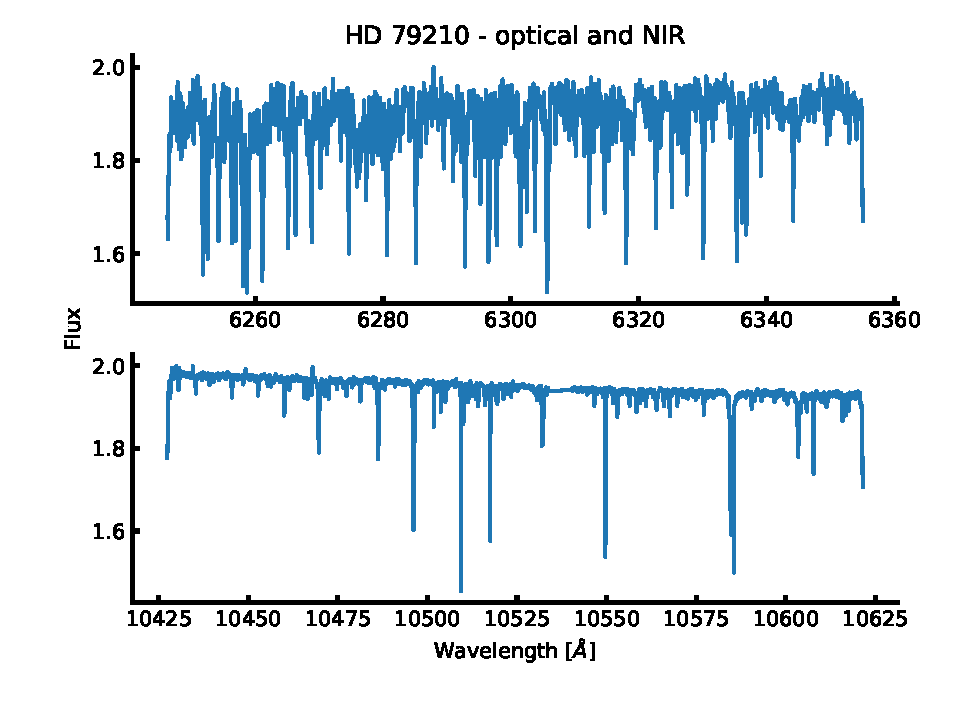
\includegraphics[width=1.0\linewidth]{figures/opticalVSnir.pdf}
    \caption{Comparison between a optical and NIR part of the spectrum of HD 79210 obtained by
             the CARMENES spectrograph. This clearly illustrate why NIR spectra are preferred over
             optical spectra for cool stars. HD 79210 is a K7 dwarf star.}
    \label{fig:opticalVSnir}
\end{figure}

The main goal of this thesis is to work towards a consistent derivation of stellar atmospheric
parameters for M stars. Before tackling the M stars, it is important to have a method that work well
for solar-like stars (FGK), which are better known during countless studies.

\subsection{Star-planet correlations}

While the stellar parameters are used to determine the planetary parameters, they can also be sued
to reveal correlations between planets and their host stars. This might give insight in the
formation and evolution of the planets. This is not a novel idea, and several correlations have been
found.

\paragraph{Giant planet and metallicity correlation}

Since the first discoveries of exoplanets, it became evident that giant planets were systematically
orbiting more metal-rich stars compared to stars with no planets. This correlation have been
confirmed by several studies \citep{Gonzalez1997,Santos2004,Fischer2005,Sousa2008a,Mortier2013b}.
This correlation in turn establish that core accretion is the main formation mechanism among giant
exoplanets \citep{Pollack1996,Ida2004,Mordasini2012} and not disc instability \citep{Boss2002}.

It is important to note that recent studies does not find this correlation for Neptune-like and
super-Earth planets \citep{Sousa2011,Buchhave2012}, thus suggesting these planets belong to a
different population.

\paragraph{Abundances of non-iron elements}

It has been shown that metal-poor stars harbouring gas planets are enhanced in alpha
elements\footnote{These are elements formed by fusion of a helium core; C, N, O, Ne, Mg, Si, S, Ar,
Ca, and Ti.} \citep[see e.g.]{Adibekyan2012a}. This means that other elements also have a role to
play in planet formation in metal poor environments. This support the core accretion theory where
planetesimals are formed from the condensation of heavy elements.


\paragraph{Lithium and the presence of planets}

It has been shown by \citep{Israelian2004,Delgado2014} that stars hosting planets are significantly
more \ion{Li}{} depleted compared to stars without planets. This correlation seems to not be
affected by different age, mass, or metallicity \citep{Sousa2010}.



\section{Applications from knowing the stars}
\label{sec:stars_application}

While ``know the star, know the exoplanet'' is the main motivation behind this thesis, it is
obviously not the only application behind detailed stellar characterisation. Working towards a
better understanding of especially M stars, which consist of to 70\% of all the stars in the Milky
Way \citep{Bochanski2010}, will also open a new window into the study of different galactic
components and galactic chemical evolution. Such a study was done by e.g. \citet{Adibekyan2012}
where spectra of 1111 FGK dwarf stars from the HARPS GTO sample was used to derive chemical
abundances of 12 refractory elements. It is possible to separate different galactic populations
(thin disk, thick disk, and the halo) by studying the chemical abundances of stars as was shown in
\citet{Adibekyan2012}.

In order to do a detailed chemical analysis as described above\footnote{See also references within
\citet{Adibekyan2012} for other similar studies.}, it is crucial to have reliable and homogeneously
derived stellar atmospheric parameters. If the parameters are homogeneously derived, i.e. with the
same method, one do not need to worry about removing possible offsets between different methods, and
in case of known offsets it is easy to correct for them (this is the case for the method used
throughout this thesis, where the surface gravity will be corrected based on another method).


\section{This thesis}
\label{sec:this_thesis}

This thesis will be focused on deriving stellar atmospheric parameters for FGK stars, making the
bridge towards M stars. The theory of stellar atmospheres in a nutshell is described in
\cref{cha:theory}, setting up all the tools to derived them as described in \cref{cha:method}. In
this chapter the description of other useful and common methods for deriving similar and different
parameters are also presented. Thereafter the knowledge will all be used in \cref{cha:results}.
First by obtaining a NIR line list containing \ion{Fe}{I} and \ion{Fe}{II} lines, then by the
derivation of parameters for HD 20010 (F sub-giant). Before deriving parameters for two K giants,
the NIR line list will be revisited.

After focusing on the NIR spectra, the optical counterpart of the method described below will be
used to derive parameters for 50 planet-host stars for an online catalogue of homogeneously derived
parameters (SWEET-Cat) in \cref{cha:SWEET-Cat}.

Last in \cref{cha:future} the future of the work established here will be discussed along with the
results already obtained. This will round of the thesis.

After the last chapter there will be an appendix with large tables that would otherwise distract the
reader from the main points. This appendix is followed by the bibliography for this thesis.
